% Created 2021-09-27 Mon 12:02
% Intended LaTeX compiler: xelatex
\documentclass[letterpaper]{article}
\usepackage{graphicx}
\usepackage{grffile}
\usepackage{longtable}
\usepackage{wrapfig}
\usepackage{rotating}
\usepackage[normalem]{ulem}
\usepackage{amsmath}
\usepackage{textcomp}
\usepackage{amssymb}
\usepackage{capt-of}
\usepackage{hyperref}
\setlength{\parindent}{0pt}
\usepackage[margin=1in]{geometry}
\usepackage{fontspec}
\usepackage{svg}
\usepackage{cancel}
\usepackage{indentfirst}
\setmainfont[ItalicFont = LiberationSans-Italic, BoldFont = LiberationSans-Bold, BoldItalicFont = LiberationSans-BoldItalic]{LiberationSans}
\newfontfamily\NHLight[ItalicFont = LiberationSansNarrow-Italic, BoldFont       = LiberationSansNarrow-Bold, BoldItalicFont = LiberationSansNarrow-BoldItalic]{LiberationSansNarrow}
\newcommand\textrmlf[1]{{\NHLight#1}}
\newcommand\textitlf[1]{{\NHLight\itshape#1}}
\let\textbflf\textrm
\newcommand\textulf[1]{{\NHLight\bfseries#1}}
\newcommand\textuitlf[1]{{\NHLight\bfseries\itshape#1}}
\usepackage{fancyhdr}
\pagestyle{fancy}
\usepackage{titlesec}
\usepackage{titling}
\makeatletter
\lhead{\textbf{\@title}}
\makeatother
\rhead{\textrmlf{Compiled} \today}
\lfoot{\theauthor\ \textbullet \ \textbf{2021-2022}}
\cfoot{}
\rfoot{\textrmlf{Page} \thepage}
\renewcommand{\tableofcontents}{}
\titleformat{\section} {\Large} {\textrmlf{\thesection} {|}} {0.3em} {\textbf}
\titleformat{\subsection} {\large} {\textrmlf{\thesubsection} {|}} {0.2em} {\textbf}
\titleformat{\subsubsection} {\large} {\textrmlf{\thesubsubsection} {|}} {0.1em} {\textbf}
\setlength{\parskip}{0.45em}
\renewcommand\maketitle{}
\author{Houjun Liu}
\date{\today}
\title{Combining Resistors Method}
\hypersetup{
 pdfauthor={Houjun Liu},
 pdftitle={Combining Resistors Method},
 pdfkeywords={},
 pdfsubject={},
 pdfcreator={Emacs 28.0.50 (Org mode 9.4.4)}, 
 pdflang={English}}
\begin{document}

\tableofcontents



\section{Combining Resistors Method}
\label{sec:org4479648}
The \href{KBhPHYS201KirkoffsLaws.org}{KBhPHYS201KirkoffsLaws}
Kirkoff's Laws themselves often requiring solving >6x6 matrixes to solve
equations quickly. Which is hard.

\subsection{Series}
\label{sec:org36223ba}
If you have two resisters\ldots{}

-----|||-----|||-----

With the first having a resistance of \(A\Omega\) and the second
\(B\Omega\).

The total resistance would simply be \((A+B)\Omega\).

\begin{itemize}
\item Same as equivalent of "electricity!" go through the first then the
second
\end{itemize}

\#disorganized

\subsection{Parallel}
\label{sec:orgc3c7925}
Smaller area |-----|||------ | Bigger area |===|||====

\(R_2 = R_1 \times \frac{A_1}{A_2}\)

\(R_{eq} = R_1 \times \frac{A_1}{A_1+A_2}\)

\(\frac{1}{R_{eq}} = \frac{A_1+A_2}{A_1R_1}\)

\(\frac{1}{R_{eq}} = \frac{1}{R_1} + \frac{A_2}{A_1R_1}\)

\(\frac{1}{R_{eq}} = \frac{1}{R_1} + \frac{1}{R2}\)

Resistance equation for series :pointup:

\noindent\rule{\textwidth}{0.5pt}

\#disorganized

Calculate resistsance

\subsection{"Combine Resistors" Method}
\label{sec:org8f632df}
\begin{figure}[htbp]
\centering
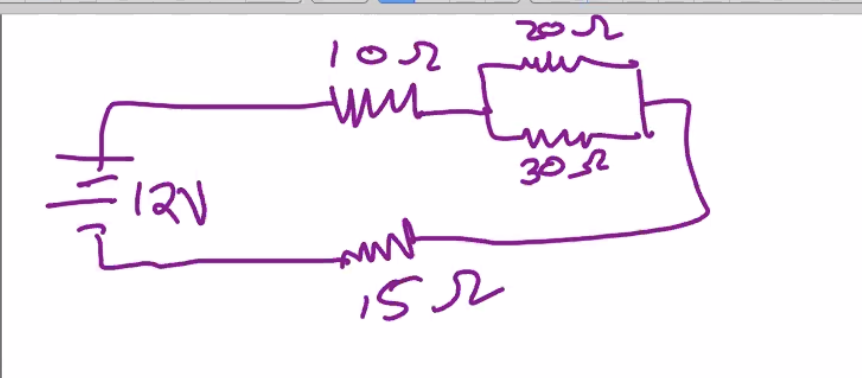
\includegraphics[width=.9\linewidth]{./Screen Shot 2020-09-14 at 11.02.45 AM.png}
\caption{Screen Shot 2020-09-14 at 11.02.45 AM.png}
\end{figure}

\subsubsection{Parallel Resistors as Single Resistors}
\label{sec:org8ffd48a}
Per the previous resisters rules, that
\(\frac{1}{R_{eq}} = \frac{1}{R_1} + \frac{1}{R2}\), we could treat the
\(20 \Omega\) and \(30 \Omega\) in parallel as a single resistor of
\(12 \Omega\).

Now the circut becomes even simpler:

\begin{figure}[htbp]
\centering
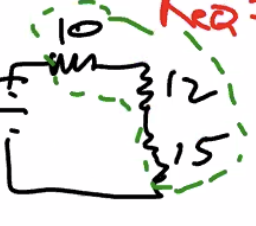
\includegraphics[width=.9\linewidth]{./Screen Shot 2020-09-14 at 11.05.49 AM.png}
\caption{Screen Shot 2020-09-14 at 11.05.49 AM.png}
\end{figure}

\subsubsection{Sequence Resistors as Single Resistors}
\label{sec:org954aaeb}
Per the sequence resisters rules, that total resistance is
\((A+B)\Omega\), we could combine these three resistors as a
\(37 \Omega\) resistor.

\subsubsection{Combined Current}
\label{sec:org06eafa0}
We know that \(12V / 37\Omega = 0.324 Amps\) is the current that returns
to the battery and what the battery starts with, for if we treat the
circuit as a single resistor, the 12 volts would only be working
against.

From there, once we have a current for beginning and end, we could work
our way up backwards by calculating the final voltage.

\begin{itemize}
\item Multiples battries can't be solved with the combined resistor method
\item So, first guess the current flow

\begin{itemize}
\item Each batteries' current will flow back to itself
\item When currents meet, they will combine
\end{itemize}

\item Use currents identified before + Kirkoff's second law
\item Use Kirkoff's first law to find loops (and hence equations) that,
together, \textbf{covers all components}
\item If resulting currents is negative, that means that you drew the
current in the wrong direction, or you are charging a battery

\begin{itemize}
\item Either way, if the signs are preserved to solve the rest of the
equation, you should be fine numerically
\item Just update your graph to reflect the actual currents' directions
\end{itemize}
\end{itemize}

LED longer leg is positive
\end{document}
